\cotefile{81}
\scanpage{42}
Soit $S$ un ens fini\inserted{Cardinal\unsure{,} $N$}, avec une structure polygonale ou \unsure{bi-circularisation} $\{u,u^{-1}\}$ ($\mathrm{Card}\,S\geq\unsure{3|2}$).

\deleted{\uline{\unsure{Déf.|Ax.}}} $T\subset S$ \inserted{de cardinal $i$} est dit un \deleted{\unsure{ens}} \uline{segment} de $S$, si

a) \deleted{\unsure{non|on}} $T\ne S$, $T\ne\varnothing$ \deleted{$\unsure{i<N}$} i.e. $0<i<N$

b) $\exists\,s_0\in S$, \deleted{$\unsure{i\in\mathbb N}$,} tel que $T=\{s_0,us_0,\ldots,u^{i-1}s_0\}$

(donc, posant $t_0={\unsure{w|u}}^{i-1}s_0$, on aura aussi $T=\{t_0,vt_0,\ldots,v^{i-1}t_0\}$, où $v=u^{-1}$).

\uline{Ex.} les parties réduites à un point.

les \unsure{parties-arêtes}.

% slanted
\margin{\deleted{\uline{\unsure{Prop.}} \unsure{Soit|Soient} $A,A'$ deux \unsure{segments},}}

$T$ est un segm. ssi $S\setminus T$ en est un.

\inserted{Intersection de deux segments \inserted{contenus dans un segment} en est un ssi il est $\ne\varnothing$}

\inserted{Réunion de deux segments pris ds un \unsure{contexte|contre-ex.}\unsure{,} et tels que \unsure{$T'\cup T''\ne S$} \inserted{est un segment}}
% slanted
\margin{\unsure{i.e.} de \deleted{\unsure{réunion}} \unsure{$\ne S$}}

Extrémités d'un segment $s_0,t_0$ (\unsure{distinctes} ssi $i\ne1$ i.e. $T$ non réduit à un point).

Origine, extrémité pour une \unsure{.} orientation.

[ \uline{NB} Si $u$ i.e. l'orientation \unsure{choisie|choisi}, le $s_0$ est unique i.e. il y a corr. \unsure{1-1|11} entre l'ens des segments de $S$, et l'ens
\[
 (S,[1,N-1]_{\unsure{\mathbb N|N}}),\ \text{via}\quad (s_0,i)\longmapsto\{s_0,us_0,\ldots u^{i-1}s_0\}.
\]

Soit $S'\subsetneq S$ une partie de $S$. Alors \deleted{les segments de $S$ contenus} deux segments de $S'$ contenus ds $S'$, et qui se rencontrent, ont comme réunion un segment \inserted{de $S$} contenu dans $S'$ -- \unsure{cela|ceci} implique
% archive sheet number: 41
\scanpage{43}
que pour tout segment $I$ de $S$, $I\subset S''$, il existe un plus grand segment de $S$ contenu dans $S'$ le contenant.

% slanted
\margin{introduire $\mathrm{Segm}_{\subset S'}(S\deleted{,\unsure{S'}})=\{I\subset S'\mid I\in\mathrm{Segm}(S)\}$}

Les éléments maximaux de $\mathrm{Segm}_{\subset S'}(S\deleted{,\unsure{S'}})$ sont appelés les \uline{segments \unsure{composants|comp.sants}} de la partie $S'$ de $S$.

% slanted
\margin{les \unsure{élém.} maximaux de $\mathrm{Segm}(S,S')$ i.e. les segments composants de $S'$, sont en corr. \unsure{1.1.} \unsure{resp.|pr.} \unsure{avec} les éléments \uline{minimaux} de l'ens des \deleted{\unsure{cl.|cl}} segments de $S$ qui \uline{contiennent} $S''$, par $I\mapsto S\setminus I$
\[
 \mathrm{Seg}_{\subset S'}(S)\overset{\unsure{\mathrm{antiiso.}}}{\simeq}\mathrm{Seg}_{\supset S''}(S)
\]}

Ils forment une partition de $S'$, d'où une relation d'équivalence dans $S'$.

En termes d'une réalisation top. de $(S,\{u,u^{-1}\})$ par un polygone top $(X,S)$, si $S''=S\setminus S'$, les \deleted{classes} segments de $S'$ sont en corr biunivoque avec les comp. conn. de $X\setminus S''$ qui rencontrent $S'$ -- ce sont les intersections de $S'$ avec ces comp. connexes.
\figure{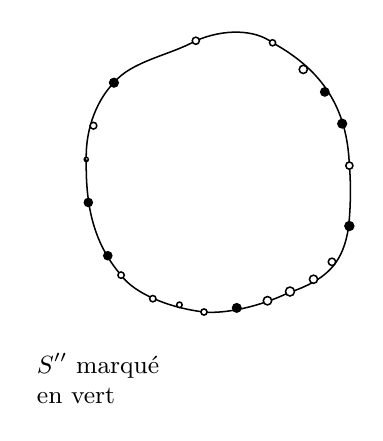
\begin{tikzpicture}[x=.013cm,y=-.013cm,line width=.55pt]
\draw (139,1183) .. controls (156,1162) and (194,1156) .. (219,1142)
 .. controls (247,1130) and (277,1131) .. (294,1144)
 .. controls (343,1171) and (367,1208) .. (369,1264)
 .. controls (371,1285) and (370,1316) .. (367,1331)
 .. controls (361,1360) and (346,1376) .. (310,1388)
 .. controls (281,1402) and (247,1409) .. (227,1407)
 .. controls (193,1403) and (159,1389) .. (146,1371)
 .. controls (121,1342) and (111,1307) .. (112,1258)
 .. controls (111,1226) and (124,1198) .. (139,1183) -- cycle;
\foreach \x/\y/\r in {219/1142/3.5,294/1144/3,324/1170/4,369/1264/3.5,352/1358/3.6,334/1375/4,311/1387/4.4,289/1396/4.1,227/1407/3,203/1400/2.7,177/1394/3.1,146/1371/3.1,119/1225/3.3}
  \draw[fill=white] (\x,\y) circle[radius=\r];
\foreach \x/\y/\r in {139/1183/5,345/1192/4.8,362/1223/5,369/1323/5.1,259/1403/4.9,133/1352/4.7,114/1300/4.7,112/1258/2.8}
  \fill (\x,\y) circle[radius=\r];
\fill[white] (112.5,1257.5) circle[radius=.8];
\node[anchor=west,align=left,font=\small] at (54,1472) {$S''$ marqué\\en vert};
\end{tikzpicture}}

\uline{Proposition} Soient $A,B$ deux parties \deleted{disjointes non vides} de $S$, on suppose \deleted{$A$ et $B$}
\[
 A,B\ne\varnothing,S,\qquad A\cap B=\varnothing.
\]

Conditions équivalentes

% slanted
\margin{\uline{NB} On peut \inserted{\unsure{prendre}} pour $\bar A,\bar B$ les \inserted{\unsure{plus|des}} \deleted{\unsure{petits}} \deleted{\unsure{segments|sgmts}} \unsure{composants|correspondants}}

a) $\exists$ segments $\bar A,\bar B$ de $S$, tels que $\bar A\supset A,\bar B\supset B$, $\bar A\cap\bar B=\varnothing$
% archive sheet number: 42
\scanpage{44}
b) Pour $a,\deleted{\unsure{b'}}a'\in A$, $b,b'\in B$, avec $a\ne a'$, $b\ne b'$, \deleted{\unsure{les ordres|les ord.}} $a,a'$ sont \deleted{\uline{contigus}} \inserted{adjacents} pour la structure \unsure{bi-circulaire|bi-circularisée} sur \inserted{l'ens à 4 éléments} $\{a,a',b,b'\}$ induite par celle de $S$, \deleted{i.e. ils} ($\Longleftrightarrow\{b,b'\}$ sont \deleted{contigus} \inserted{adjacents} $\Longleftrightarrow\{a,a'\}$ ne sont pas opposés $\Longleftrightarrow b,b'$ ne sont opposés

c) $B$ est contenu dans un segment composant de $S\setminus A$

c$'$) $A$ est contenu dans un segment composant de $S\setminus B$

% slanted
\margin{d) Quand $S$ est réalisé comme \inserted{partie} d'un disque \inserted{convexe} plongé dans un plan réel affine)\,: Soit $P_A$ la réunion des segments affines joignant deux à deux les points de $A$ (ou, \unsure{au choix|au besoin}, l'enveloppe convexe de $A$) alors $P_A\cap P_B=\varnothing$}

Quand il en est ainsi, parmi les couples $(\bar A,\bar B)$ \inserted{de segments} satisfaisant les conditions de a), il existe un plus petit\ldots

On dit que $A,B$ sont \uline{non panachés}

(\uline{Ex} Si \deleted{\unsure{$A$ et}} $A$ ou $B$ réduit à un pt. \inserted{(\unsure{plus généralt|plus généralmt} si $A$ ou $B$ est un segment}

Si $A$ et $B$ sont de cardinal 2, cel. signifie que, sur $A\cup B$ pour la bicircularisation induite, $A$ est un côté du carré $A\cup B$ (i.e. encore que $B$ est un côté). Dans le cas général, $A$ et $B$ sont non panachés ssi $\forall\, A'\in\unsure{P_2|\mathcal P_2}(A)$, $B'\in P_2(B)$, $A'$ et $B'$ sont non panachés.

% slanted
\margin{\deleted{e) \unsure{On a} $A,B\subset C$, \unsure{$C=$|un} segment \unsure{on a des} $\bar A,\bar B$ \unsure{ds|de} \unsure{st} $\bar A\cap\bar B=\varnothing$, \unsure{$=\ A$}}}

% slanted
\margin{\uline{Cor} De plus, \unsure{lorsque ces} conditions \unsure{sont} \unsure{sauf} dans le cas où $A\mathbin{\unsure{\sqcup|\cup}}B=S$ (\unsure{donc|alors} $A$ et $B$ des segments compl. l'un de l'autre), \unsure{quand il} existe \inserted{donc} un segment $C\supset A\cup B$, on peut prendre pour $\bar A,\bar B$ ds a) les \unsure{composantes de $A$ et $B$|composants de $A$ et $B$} $\subset C$.}
% archive sheet number: 43
\scanpage{45}
\uline{Structure à étudier} Partition de $S$ en des $(S_\alpha)_{\alpha\in\unsure{J|I}}$ mutuellement non panachées. (On les appelle des partitions non \unsure{panachées|panachés})

% slanted
\margin{\uline{Ex} \unsure{partition|partitions} \unsure{grossière|grossières}, \unsure{ayant} \unsure{juste} une classe, égale à $S$\unsure{\ldots|--}}

\uline{Intuition} À \deleted{\unsure{une tel|un tel}} un ens. bicircularisé avec partition non panachée, \inserted{de \deleted{\unsure{Card.}} \unsure{cardinal|Cardinal} $N$,} correspond (\unsure{fonctoriellement} pour les \unsure{iso}) un ens. bicircularisé (d'\deleted{ordre} cardinal \inserted{\uline{pair}} $N'\leq N$), avec une partition \inserted{non panachée} de degré 2 (classes de cardinal 2).\unsure{\,--|\ldots}

\figure{\begin{tikzpicture}[x=.011cm,y=-.011cm,line width=.65pt]
\draw (578,1785) .. controls (632,1751) and (637,1702) .. (664,1620)
 .. controls (685,1547) and (706,1482) .. (670,1401)
 .. controls (632,1315) and (543,1273) .. (449,1281)
 .. controls (366,1284) and (291,1314) .. (225,1374)
 .. controls (173,1424) and (162,1475) .. (158,1544)
 .. controls (144,1612) and (168,1680) .. (195,1725)
 .. controls (254,1806) and (355,1865) .. (428,1858)
 .. controls (487,1855) and (556,1837) .. (601,1781);
\end{tikzpicture}}
% archive sheet number: 44
\scanpage{46}
Soit $\Sigma$ un ens. de segments de $S$, satisfaisant la condition suivante

($\deleted{\unsure{\Sigma|>}}\sigma$ 1) Si $A,B\in\Sigma$, et si $A\cap B\ne\varnothing$, alors $A\subset B$ ou $B\subset A$. \inserted{($\sigma.2$)} Si de plus $A\ne B$ et $A\subset B$, alors $A$ ne contient pas d'extrémité de $B$.

Posons alors, pour $A\in\Sigma$
\[
 A^*=\unsure{.|\cdot}\, A\setminus\bigcup_{\substack{B\in\Sigma\\ B\subset A\\ B\ne A}} B
\]
On a (par $\sigma.2$)
\[
 A^*\supset\partial A\quad\text{(ens des extrémités de $A$)}
\]
donc $A^*\ne\varnothing$. Je dis que
\[
 \begin{aligned}
 A&\longmapsto A^*\\
 \Sigma&\longrightarrow \unsure{P|\mathcal P}(S)
 \end{aligned}
 \qquad\text{est injectif}
\]
% slanted
\margin{\uline{Prop} Si $A,B\in\Sigma$, $A\ne B$, alors $A^*\cap B^*=\varnothing$ (donc $A^*\ne B^*$), \deleted{\unsure{sont disj.|sont di}} et $A^*,B^*$ non panachés. On a $\bigcup_{A\in\Sigma} A=\bigcup_{A\in\Sigma} A^*$. Si $x\in\bigcup_{A\in\Sigma}A$, alors \unsure{l'ens|l'ens.}\inserted{$\Sigma\unsure{(x)|^{(x)}}$} des $A\in\Sigma$ tels que $x\in\Sigma$ est \unsure{tot.} ordonné, donc admet un plus petit élément, soit $A$, et alors $A^*\unsure{\ni|\to}x$.}
i.e. que si $A,B\in\Sigma$, alors
\[
 A^*=B^*\quad\Longrightarrow\quad A=B
\]
\inserted{i.e. $A\ne B$ \deleted{distincts} $\Longrightarrow A^*\ne B^*$. Comme $A^*,B^*$ sont $\ne\varnothing$, il suffit de prouver $A^*\cap B^*=\varnothing$.} \deleted{En effet}, si $A\cap B=\varnothing$, alors $A^*\cap B^*=\varnothing$, donc $A^*\ne B^*$ (puisque $A^*,B^*$ non vides). Si $A\cap B\ne\varnothing$, on a \inserted{(par $\sigma\,1$)} $A\subset B$ ou $B\subset A$, soit $A\subset B$.

\deleted{Mais alors $A\cap\partial B=\varnothing$ \inserted{par $\sigma 2$}, donc $A^*\cap\partial B=\varnothing$, donc \unsure{$A^*\supset$|$A\supset$} (comme $\varnothing\ne\partial B\subset B^*$) $A^*\not\supset B^*$. Or \unsure{on aurait|on a} $A^*\cap\partial B=$} Comme $A\ne B$, $A\cap B^*=\varnothing$ par définition de $B^*$, donc $A^*\cap B^*=\varnothing$, cqfd. \deleted{Je dis} Aussi, $A^*,B^*$ non panachés, puisque $A^*\subset A$ segment $\subset S\setminus B^*$.
% archive sheet number: 45
\scanpage{47}
\uline{Conséquence}: Si $\bigcup_{A\in\Sigma}A^*=S$, alors \deleted{les} $(A^*)_{A\in\Sigma}$ est une partition \deleted{\unsure{des|sans}} \unsure{non} panachée de $S$. Si $\bigcup_{A\in\Sigma} A^*\ne S$, alors posant
\[
 \deleted{\unsure{R,\Sigma|R\ \Sigma}}\mathpunct{.}\qquad
 \left\{\begin{aligned}
 R&=S\setminus\bigcup_{A\in\Sigma}A^*\\
 R^*&=R\setminus\bigcup_{\substack{A\in\widehat\Sigma\\ A\ne R}}A=R
 \end{aligned}\right.,\qquad
 \begin{aligned}
 \widehat\Sigma&=\Sigma\cup\{R\}\\
 &\deleted{\unsure{\Sigma|\in\Sigma}}
 \end{aligned}
\]
alors $(A^*)_{A\in\widehat\Sigma}$ est une partition non panachée de $S$.

\uline{NB} Si $R$ est lui-= un segment, alors \deleted{\unsure{l'intérêt} \unsure{de le prendre|de le joindre}} $\widehat\Sigma$ satisfait les conditions de $\Sigma$ -- et $R$ est un élément \deleted{``\unsure{sp.|spéc.}} ``isolé'' de $\widehat\Sigma$, \unsure{en|au} ce sens que \inserted{pour} \unsure{tt|$A$} autre élément \inserted{$A$} de $\widehat\Sigma$, \deleted{\unsure{on}} \unsure{.} $R\cap A=\varnothing$ -- \deleted{\unsure{donc}} \inserted{i.e.} $R$ est \unsure{à|:} la fois minimal, et maximal. Considérons
\begingroup
\makeatletter\tagsleft@true\makeatother
\[
 \tag*{$(\sigma\ 3)$}
 \begin{aligned}
 R=S\setminus\bigcup_{A\in\Sigma}A\;
 \bigl(=S\setminus\bigcup A^*\bigr)&\quad\text{n'est}\\
 &\quad\text{pas un segment}
 \end{aligned}
\]
\endgroup
(NB \unsure{c'est} le cas si $R=\varnothing$ \unsure{p. ex|p. ex.})

% slanted
\margin{faux}
Montrons dans ce cas \unsure{que} \deleted{\unsure{on a|est}} $\Sigma$ est \deleted{défini} \inserted{\unsure{connu|connus}} quand on connait la partition $\widehat\Sigma^*=\{A^*\mid A\in\widehat\Sigma\}$

\[
 \bigl(\text{où }\widehat\Sigma=\left\{\begin{aligned}
 &\Sigma\quad\text{si }R=\varnothing\\
 &\Sigma\cup\{R\}\quad\text{si }R\ne\varnothing
 \end{aligned}\right.\bigr)
\]
% archive sheet number: 46
\scanpage{48}
Je veux caractériser $A$ en termes de $\widehat\Sigma^*, A^*\in\widehat\Sigma^*$ (dans le cas $A\in\Sigma$). Bien sûr, $A$ est un \deleted{\unsure{segt|segt.}} segment qui contient $A^*$, et comme $A^*\supset\partial A$, il est minimal (\deleted{\unsure{l'unique|l’un}} \unsure{qui convient|pas uniquement}) parmi les segments \inserted{de $S$} qui conti\deleted{\unsure{ent}}ennent $A^*$ -- mais cela ne suffit pas à le caractériser. Il a cependant la propriété supplémentaire,
\[
 \forall B^*\in\widehat\Sigma^*,\quad\text{on a}\quad B^*\cap A=\varnothing,\quad\text{ou }B^*\subset A
\]

\uline{NB} En fait, avec les seules conditions $\sigma1$ \unsure{à|:} $\sigma3$ sur $\Sigma$, \deleted{\unsure{c'|i}} il n'est pas vrai que la connaissance de $\widehat\Sigma^*$ redonne $\Sigma$, exemple

\figure{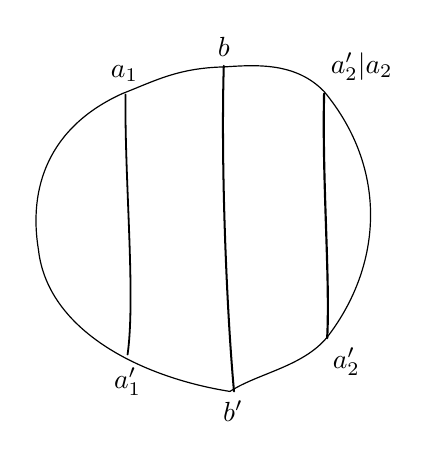
\begin{tikzpicture}[x=.013cm,y=-.013cm,line cap=round,line join=round]
\draw[line width=.43pt] (232,1287) .. controls (159,1320) and (140,1380) .. (150,1440) .. controls (159,1518) and (249,1564) .. (337,1578) .. controls (365,1560) and (408,1554) .. (432,1525) .. controls (486,1455) and (492,1361) .. (429,1285) .. controls (401,1256) and (362,1259) .. (331,1261) .. controls (286,1262) and (263,1275) .. (232,1287);
\draw[line width=.65pt] (235,1288) .. controls (234,1372) and (245,1485) .. (237,1542);
\draw[line width=.73pt] (331,1260) .. controls (328,1360) and (334,1502) .. (341,1578);
\draw[line width=.78pt] (429,1287) .. controls (427,1374) and (435,1468) .. (432,1526);
\node[above] at (234,1285) {$a_1$};
\node[above] at (331,1260) {$b$};
\node[above right] at (426,1284) {$\unsure{a'_2|a_2}$};
\node[below] at (237,1545) {$a'_1$};
\node[below] at (340,1578) {$b'$};
\node[below right] at (428,1526) {$a'_2$};
\end{tikzpicture}}
relation d'équiv. \inserted{$\unsure{\mathcal R|R}$} avec trois classes $\{a_1,a'_1\}$ $\{b,b'\}$ $\{a_2\unsure{,|{}}a'_2\}$, \inserted{\unsure{définir ici|définissons}} $\Sigma_1$ formé des segments $\{a_i,a'_i\}$ \deleted{$\unsure{\{a,a'\}|\{a_i,a'_i\}}$} $(i\in\{1,2\})$, et $\{a_1,a'_1,b,b'\}$ et $\Sigma_2$ défini de façon symétrique, définissent la $=$ $\mathcal R$\unsure{.|*}

% Four long diagonal cancellation strokes run through the following block.
\deleted{\unsure{Exemple|Énoncé} plus général: on peut de façon unique \unsure{trouver|choisir} $\Sigma$ de façon à donner}
\[
 \begin{aligned}
 &\left\{\begin{aligned}
   &\deleted{\widehat\Sigma^*=\unsure{\mathcal R|\mathcal A},\quad\text{\uuline{et}}}\\
   &\deleted{\unsure{\dot R|R}\overset{\text{déf}}{=}S\setminus\coprod_{A\in\Sigma} A=\unsure{S'|S_1|S_i},}
 \end{aligned}\right.\\
 &\qquad\deleted{\text{élément \uline{donné} d'}}\\
 &\qquad\deleted{\text{avance de }\mathcal R}\\
 &\qquad\deleted{\text{\unsure{$S'$|si} non un segment}}
 \end{aligned}
\]
% archive sheet number: 47
